
\documentclass[12pt, a4paper, twoside]{article}
\usepackage[utf8]{inputenc}
\usepackage[english]{babel}
\usepackage{cite}
\usepackage{graphicx}
\usepackage{color}
\usepackage{amsmath}
\usepackage{amssymb}
\usepackage{graphicx}  
\usepackage{subcaption}
\usepackage{url}
\usepackage{float}
\usepackage[dvipdfm]{hyperref}

\title{Biomedical Signal Display}
\author{Jinu Jayachandran}
\date{December 2017}
 
\begin{document}
 
\begin{titlepage}
\maketitle
\end{titlepage}

\section{Introduction}
    The display of signals generated by various sources in an efficient manner is of great importance in the field of research. There are instruments which can display the signals at different levels of accuracy. The more accurate the instrument is the more costlier it becomes and the relationship is exponential. Also the range of frequency of signals (or in other words the bandwidth of the signals) is also an important factor. But is it possible to make an in-house display for relatively small frequency signals using minimum components and less cost?. This possibility is being explored in the project. The scope of the project is mainly confined to displaying biomedical signals which will range only in hundreds of frequency. Also the project aims to display two signals at the same time.
    
\section{The System}
    For the display of analog signals the three important components needed are the sampler, the processing unit and the display. The system can also be designed in such a way that sample-processing unit will itself form a single entity or even better, all three are in the single system. In this project all the three are three different units and are handled individually. 

\subsection{Analog to Digital Converter (ADC)}
    An ADC will perform the function of a sampler. Depending on the range of signals to be displayed an appropriate ADC can be chosen. By 'appropriate' it means that a decision should be made on what should be the sampling time (or speed), resolution, voltage range, interface type etc of the ADC. Currently in the first phase of the project ADC is not used. Instead the waveform to be displayed is generated in the processing unit and sent to the display.

\subsection{Processing Unit}
    The three main tasks of the processing unit are - Receive data, Process data and Send data to display. The data that is being received from the ADC can be through an interface. The interface can be a serial interface like UART, SPI, I2C etc or a parallel one. To process data received there should be a unit which can analyze the data and modify it so that it can be displayed suitably. Thus a microcontroller is one of the choices of the processing unit. In this project we are using \href{https://www.raspberrypi.org/}{Raspberry Pi Rev2.0}\cite{bib_raspberrypi}  is used as the processing unit. Fig(\ref{fig_rpi}) shows the Raspberry Pi Rev 2.0 Model B which is used in the current project.
 
\begin{figure}[ht]
    \centering
    %\scalebox{0.5}{\input{./fig/rpi.pstex_t}}
    \includegraphics[scale=0.75]{./fig/rpi.ps}
    \caption{Raspberry Pi}
    \label{fig_rpi}
\end{figure}

The Raspberry Pi can be considered as a minicomputer with lot of interfaces. Even a monitor and keyboard can be attached to pi and can be used as a normal computer. But the resources to the pi are limited. The only memory it can have is via an SD Card. The pi can only work with a custom OS. The most commonly used OS is raspbian \cite{bib_raspbian}

The display that is used is \href{http://www.4dsystems.com.au/product/uLCD_32PTU/}{uLCD-32PTU} from 4D systems \cite{bib_ulcd}

\bibliographystyle{plain}
\bibliography{dso}
 
\end{document}


